% !TeX root = relazione.tex
\documentclass{article}

\usepackage[utf8]{inputenc}
\usepackage[a4paper, total={15.3 cm, 21.3 cm}]{geometry}
\usepackage{amsmath}
\usepackage{amssymb}
\usepackage{gensymb}
\usepackage{booktabs}
\usepackage{hyperref}
\usepackage{caption}
\usepackage{float}
\usepackage{graphicx}
\usepackage{subfig}
\usepackage{titlesec}
\usepackage{titletoc}
\usepackage{physics}
\usepackage{siunitx}
\usepackage[dvipsnames]{xcolor}

\usepackage{longtable}
\usepackage{tabularx}
\usepackage{calc}
\usepackage{array}
\usepackage{subfiles}
\usepackage{etoolbox}
\usepackage{xparse}


\hypersetup{colorlinks=true,linkcolor=black}
\renewcommand\thesection{\arabic{section}}
\titlecontents{chapter}[1.05em]{\bigskip}
{\contentslabel[\MakeUppercase{\romannumeral\thecontentslabel}]{1em}\enspace\textsc}
{\hspace*{-1em}\textsc}
{\hfill\contentspage}
\titlecontents{section}[1.6em]{\smallskip}
{\thecontentslabel.\enspace}
{}
{\titlerule*[1pc]{.}\contentspage}
\setcounter{tocdepth}{2}


\begin{document}

    \pagenumbering{roman}
    \thispagestyle{empty}

    % First page with uni logo and title
    \begin{center}

        
\includegraphics[width=1.\linewidth]{../../../tools/images/logo.jpg}
        \centering
        \vspace{3cm}

        \uppercase{\Large Relazione di laboratorio:\\ misura della velocità della luce\par}
        \vspace{3cm}

        \Large Lorenzo Liuzzo, Jiahao Miao, Riccardo Salto\par
        \vspace{1.5cm}

        \Large Novembre 23, 2022

    \end{center}

    \clearpage

    % Table of contents
    \tableofcontents

    \clearpage
    \pagenumbering{arabic}

    % Abstract con una breve descrizione dell'esperimento e i risultati
    \section{Abstract}
    
        È stato utilizzato uno spettrometro a reticolo per misurare le lunghezze d'onda di alcune righe dello spettro di
        emissione di una lampada ai vapori di mercurio sfruttando il fenomeno fisico della diffrazione. Nell'arco dell'esperimento 
        sono stati inoltre valutati il potere dispersivo $D$ e il potere risolutivo del reticolo $R$ per ogni ordine $k$.\\
        Nella tabella \ref{tabular:Lambda spettro} sono riportale le lunghezze d'onda $\lambda$ con l'errore associato $\sigma_{\lambda}$,
        mentre in figura \ref{fig:Distriduzione spettro} è possibile osservare 
        l'intera distribuzione dello spettro del mercurio. 
        Riportiamo nella tabella \ref{tabular:Parametri strumento} anche i valori delle grandezze caratteristiche dell'apparato 
        calcolati con la lampada al sodio.  
        
        \begin{table}[H]

            \centering
            \begin{tabular}{c c c}

                \toprule 

                \textbf{colore}                     &  \textbf{$\lambda$ [nm]}  & \textbf{$\sigma_{\lambda}$ [nm]} \\

                \midrule

                \textcolor{purple}{Viola int.}	         &	   404,0	    &	  0,4                 \\
                \textcolor{violet}{Viola est.}           &	   406,8	    &	  0,4                 \\
                \textcolor{cyan}{blu}                    &	   434,8	    &	  0,4                 \\
                \textcolor{Aquamarine}{Verde acqua int.} &	   490,9	    &	  0,5                 \\
                \textcolor{Emerald}{Verde acqua est.}	 &	   496,9	    &	  0,5                 \\
                \textcolor{green}{Verde}                 &	   545,6	    &	  0,5                 \\
                \textcolor{Goldenrod}{Giallo int.}     	 &	   575,2	    &	  0,6                 \\
                \textcolor{yellow}{Giallo est.}	         &	   578,1	    &	  0,6                 \\
                \textcolor{red}{Rosso int.}              &	   616	        &	  1                   \\
                \textcolor{BrickRed}{Rosso est.}         &	   618 	        &	  1                   \\

                \bottomrule
        
            \end{tabular}

            \caption{Lunghezze d'onda dello spettro del mercurio}
            \label{tabular:Lambda spettro}

        \end{table}

        \begin{table}[H]

            \centering

            \begin{tabular}{c c}

                \toprule 

                \textbf{Parametro} & \textbf{Valore}    \\

                \midrule

                $L$  & $(25\ \pm \ 1)\, \mathrm{mm}$    \\
                $d$  & $(3,369 \pm 0,002)\, \mathrm{\mu m}$    \\
                $N$  & $(7,5 \pm 0,1) \cdot 10^3$           \\
                $D$  & $(5,454 \pm 0,005) \cdot 10^5 \, \mathrm{rad/m}$   \\
                
                \bottomrule

            \end{tabular}

            \caption{Parametri strumento}
            \label{tabular:Parametri strumento}
            
        \end{table}

        \begin{figure}[H]

            \centering
            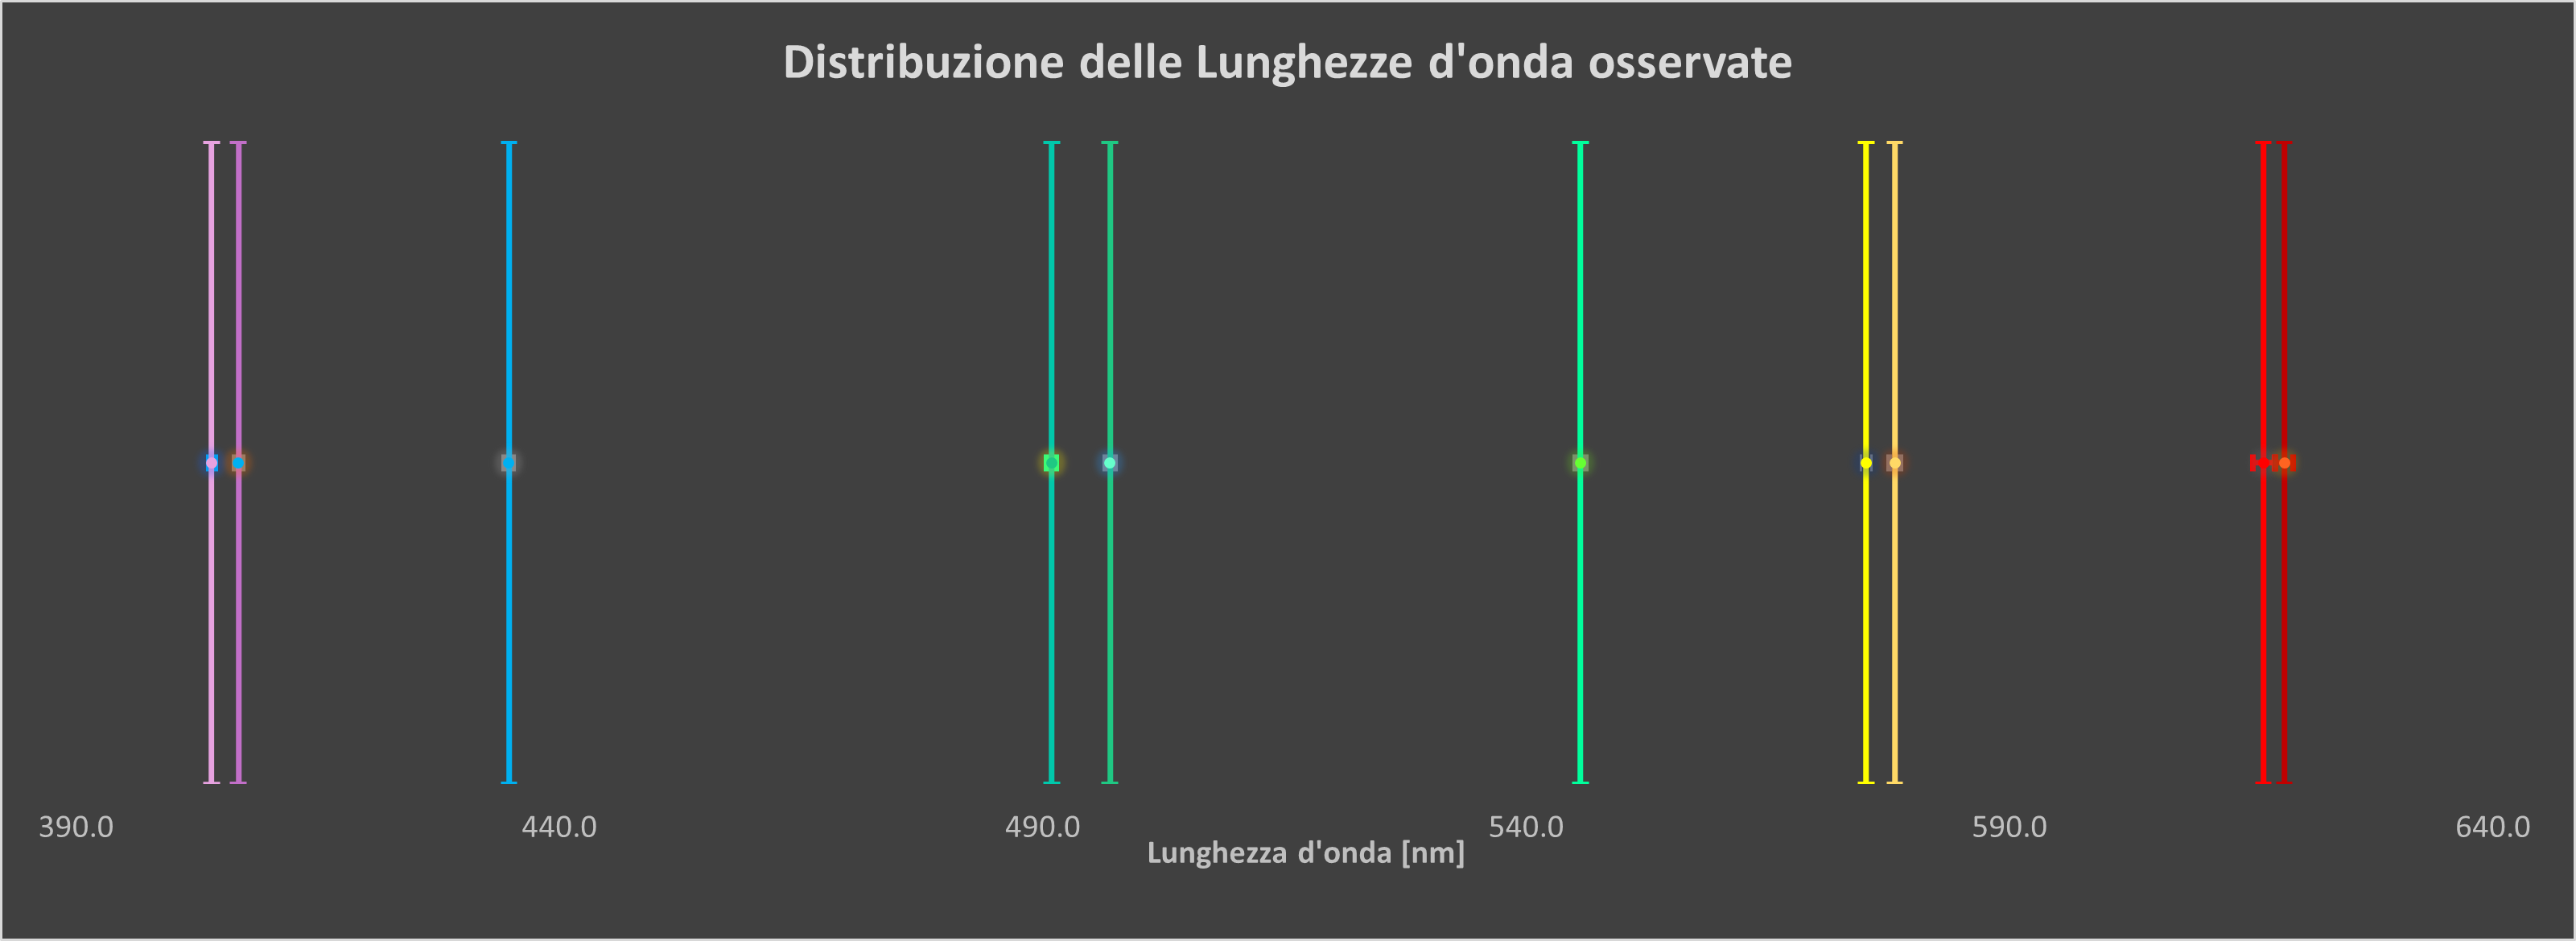
\includegraphics[width = 15cm]{../images/spettro.png}
            \caption{Distribuzione delle righe della lampada ai vapori di mercurio osservata in laboratorio}
            \label{fig:Distriduzione spettro}
            
        \end{figure}
       
    
    \section{Calibrazione dell'apparato}

        Innanzitutto si è proceduto con la messa a fuoco del cannocchiale rispetto a un obbiettivo sufficientemente lontano affinchè 
        fosse valida l'approssimazione di onda piana. A questo punto è stato messo a fuoco il collimatore rispetto alla precedente regolazione
        del cannocchiale in modo che fosse verificata l'approssimazione di campo lontano. La piattaforma che regge il reticolo è stata poi messa in bolla. \\
        Con una lampada ai vapori di sodio è stato ortogonalizzato il reticolo rispetto all'onda piana, dopo aver regolato l'apertura della fenditura 
        in modo da osservare righe sufficientemente sottili e luminose (larghe all'incirca $0.5$ mm). 
        L'ortogonalizzazione è stata effettuata attraverso la misura delle posizioni angolari relative allo zero del medesimo ordine di interferenza 
        di una riga del doppietto del sodio a sinistra e a destra dell'ordine centrale.
        È stato poi calcolato l'angolo di correzione $\beta$, tramite la relazione:
            \[ \beta = \frac{\theta_2 - \theta_1}{2} \cdot \frac{\cos(\theta_{av})}{1 - \cos\theta_{av}} \]
        dove $\theta_1$ e $\theta_2$ sono le posizioni angolari delle righe del sodio, $\theta_{av}$ è invece la media delle due. \\
        A questo punto, il reticolo è stato ruotato dell'angolo $\beta$ ed è stata ripetuta la misura. La procedura è stata eseguita due volte prima di 
        ottenere una precisione di $4'$, inferiore alla precisione minima richiesta di $5'$. \\ 


    \section{Valutazione delle grandezze caratteristiche dell'apparato}

        Si è proceduto con la determinazione dei parametri caratteristici del reticolo e delle lunghezze d'onda associate allo spettro del mercurio. \\
        Innanzitutto è stata misurata la lunghezza $L$ del reticolo con un righello di risoluzione $1$ mm: \[L = (25\ \pm \ 1)\, \mathrm{mm}\]
        Tutte le misurazioni delle posizioni angolari dei massimi di interferenza sono invece state effettuate su un nonio con risoluzione di $1'$ e 
        successivamente  convertite in radianti. Come incertezza associata alla singola misura è stata utilizzata la risoluzione dello strumento
        $\sigma = 0.02$ ° $ = 3\cdot10^{-4}$ rad.
        Dunque è stata stimata la posizione angolare dell'ordine centrale $\theta_0$ osservandola sul nonio. La misura è stata ripetuta 6 volte 
        e con una media è stato ricavato il valore migliore. Come incertezza è stata scelta comunque la risoluzione dello strumento, 
        poichè maggiore della deviazione standard: \[\theta_0 = (56,07 \pm 0.02) ^{\circ} = (0.9786	\pm 0.0003 )\, \mathrm{rad}\]
        In seguito, note le lunghezze d'onda del doppietto del sodio, $\lambda_{{Na}_1} = 589.0\ \mathrm{nm}$ e $\lambda_{{Na}_2} = 589.6\ \mathrm{nm}$,
        sono state misurate le posizioni angolari dei massimi di interferenza per i primi 5 ordini riferiti a $\lambda_{{Na}_1}$. 
        Per ogni ordine $k$, l'angolo $\theta_k$ è stato valutato come differenza tra il valore letto sul nonio e $\theta_0$. 
        L'errore associato $\sigma_{\theta_k}$ è stato valutato come somma in quadratura di due differenti errori $\sigma_s$ e $\sigma_o$; 
        il primo è a sua volta la somma in quadratura delle due incertezze associate alla singola misura angolare $\sigma_{\theta}$, 
        il secondo legato all'errore di ortogonalizzazione e ricavato dalla formula: \[\sigma_o = \beta \cdot \frac{1-cos(\theta_k)}{cos(\theta_k)}\]
        Dopo aver convertito in radianti le grandezze appena descritte ne è stato calcolato il seno con il suo errore associato $\sigma_{sin(\theta_k)}$,
        ricavato dalla formula di propagazione: \[\sigma_{sin(\theta_k)} = \sigma_{\theta_k} \cdot |cos(\theta_k)|\] \\
        In tabella \ref{tabular:posizioni angolari sodio} sono riportati i valori misurati per le posizioni angolari e i valori di $\sin(\theta_k)$.
        \begin{table}[H]

            \centering

            \begin{tabular}{c c c c}

                \toprule 
                $\theta_k$° & $sin(\theta_k)$ & $\sigma_{sin(\theta_k)}$ & k \\
                
                \midrule
                10,06	&	0,17	&	0,02	&	1\\
                20,54	&	0,35	&	0,03	&	2\\
                30,93	&	0,51	&	0,04	&	3\\
                45,28	&	0,71	&	0,07	&	4\\
                63,68	&	0,9	    &	0,1	    &	5\\
                \bottomrule
            
            \end{tabular}
            
            \caption{Posizioni angolari $\lambda_1$ rispetto agli ordini k}
            \label{tabular:posizioni angolari sodio}

        \end{table}

        A questo punto, per ogni ordine $k$ è stato ricavato il passo del reticolo $d$ e la sua incertezza $\sigma_d$ dalle formule: 
        \[d = \frac{\lambda_1 \cdot k}{sin(\theta_k)} \ \ \ \sigma_d = \frac{d \cdot \sigma_{\theta_k}}{|tan(\theta_k)|}\]
        e da questo il numero di fenditure $N$ e la sua incertezza $\sigma_N$: 
        \[N = \frac{L}{d} \ \ \ \sigma_N = N \sqrt{(\frac{\sigma_L}{L})^2 + (\frac{\sigma_d}{d})^2}\]
        dove $\sigma_L$ è l'incertezza associata alla lunghezza $L$ del reticolo. \\
        
        In tabella \ref{tabular:passo reticolo e N} sono riportati i valori di $d$ e $N$ per i 5 ordini. 
        \begin{table}[H]

            \centering

            \begin{tabular}{c c c c c}

                \toprule 
                $k$ & $d$ [m] & $\sigma_d$ [m]  &  $N$  &   $\sigma_N$ \\
                
                \midrule
                1 & 3,372E-06	&	8E-09	&	7E+03   &   3E+02    \\
                2 & 3,357E-06	&	4E-09	&	7E+03   &   3E+02    \\
                3 & 3,438E-06	&	4E-09	&	7E+03   &   3E+02    \\
                4 & 3,316E-06	&	5E-09	&	8E+03   &   3E+02    \\
                5 & 3,286E-06	&	8E-09	&	8E+03   &   3E+02    \\
                \bottomrule
                
            \end{tabular}

            \caption{Passo del reticolo d e numero di fenditure N}
            \label{tabular:passo reticolo e N}

        \end{table}
  
        È stato poi valutato il potere dispersivo $D$ e l'incertezza $\sigma_D$: 
        \[D = \frac{k}{d \cdot cos(\theta_k)} \ \ \ \sigma_D = D \cdot \sqrt{(\frac{\sigma_d}{d})^2 + (\sigma_{\theta_k} \cdot tan(\theta_k))^2}\]
        Infine è stato calcolato il potere risolvente $R$ e il suo errore $\sigma_R$ dalle relazioni: \[R = k \cdot N \ \ \ \sigma_R = \sigma_N \cdot k\] \\ 
        
        In tabella \ref{tabular:potere dispersivo e risolutivo} sono riportati per ogni ordine $k$ il potere dispersivo e risolutivo associati e con relativa incertezza. 
        \begin{table}[H]

            \centering

            \begin{tabular}{c c c c c }

                \toprule 
                $k$ & $D $[rad/m]  & $\sigma_D$ [rad/m] & $R$ & $\sigma_R$  \\
                \midrule
                1	&	3,012E+05	&	7E+02	&	7,4E+03	    &	3E+02   \\
                2	&	6,363E+05	&	8E+02	&	1,49E+04	&	6E+02   \\
                3	&	1,017E+06	&	1E+03	&	2,2E+04	    &	1E+03   \\
                4	&	1,714E+06	&	4E+03	&	3,0E+04	    &	1E+03   \\
                5	&	3,43E+06	&	2E+04	&	3,8E+04 	&  	2E+03   \\
                \bottomrule
        
            \end{tabular}

            \caption{Potere dispersivo e risolutivo del reticolo per ogni ordine}
            \label{tabular:potere dispersivo e risolutivo}

        \end{table}
        

    \section{Misura delle lunghezze d'onda dello spettro del mercurio}

        Una volta cambiata la lampada al sodio con una ai vapori di mercurio, si è proceduto con la misura indiretta delle lunghezze d'onda del suo spettro.
        Le misure sono state ripetute allo stesso modo per ogni colore. Sono stati osservati i seguenti colori: viola interno, viola esterno, indaco, 
        verde acqua interno, verde acqua esterno, verde, giallo interno, giallo esterno, rosso interno (è stato osservato solo il primo ordine destro e sinistro), 
        rosso esterno (è stato osservato solamente l'ordine 1 e 2 destro). \\
        Partendo dal primo ordine (destro o sinistro indifferentemente) è stata misurata col nonio la posizione angolare della banda del colore prescelto
        fino al terzo ordine. La misura è poi stata ripetuta dall'altra parte. Per le misure angolari si è proceduto come già fatto per la lampada al sodio,
        per cui i valori degli angoli $\theta_k$ sono stati convertiti in radianti, ne è stato calcolato il seno, e gli errori sono stati propagati come sopra.
        Le lunghezze d'onda $\lambda_k$ dei singoli colori sono state ricavate dalla relazione: \[\lambda_k = \frac{d sin(\theta_k)}{k}\]
        L'errore associato $\sigma_{\lambda_k}$ è stato invece valutato con la seguente formula di propagazione:
        \[\sigma_{\lambda_k} = \lambda_k \sqrt{(\frac{\sigma_d}{d})^2 + (\frac{\sigma_{\theta_k}}{tan(\theta_k)})^2}\]
        nella quale tutte le quantità sono state precedentemente definite. 
        In Appendice \ref{Appendice} sono riportate le tabelle con i valori di $k$, $\theta_k$, $sin(\theta_k)$, $\lambda_k$ con relativi errori per ogni colore osservato. 
        I risultati finali delle lunghezze d'onda $\lambda$ per ogni colore sono stati ottenuti con una media pesata dei $\lambda_k$, 
        dove all'errore è stato sommato in quadratura l'errore di ortogonalizzazione $\sigma_{\lambda_o}$ ricavato dalla formula:
        \[\sigma_{\lambda_o} = \lambda \frac{\sigma_d}{d} \]
        

    \section{Potere dispersivo del reticolo calcolato a partire dai dati raccolti sulle lunghezze d'onda}
        
        È stato infine calcolato il potere dispersivo del reticolo per i primi tre ordini $k$ a partire dai dati raccolti sulle lunghezze d'onda.
        La procedura è stata ripetuta per ogni ordine considerato. Sono state quindi considerate le tre coppie di viola, gialli e verdi acqua. 
        Per ogni doppietto è stata valutata la distanza angolare $\Delta \theta$ tra le posizioni angolari dei massimi dello stesso ordine dei due colori vicini 
        (riportate in Appendice \ref{Appendice}) e la differenza tra le loro lunghezze d'onda $\Delta \lambda$ (riportate in tabella \ref{tabular:Lambda spettro}). 
        Gli errori sulle grandezze di $\Delta \theta$ e $\Delta \lambda$ sono stai stimati con una somma in quadratura dei singoli errori sulle posizioni angolari e
        sulla stima delle lunghezze d'onda. A questo punto è stato valutato il potere dispersivo $D$ secondo la formula: \[D = \frac{\Delta \theta}{\Delta \lambda}\]
        L'errore associato $\sigma_D$ è stato invece valutato come:
        \[\sigma_D = D \sqrt{(\frac{\sigma_{\Delta \theta}}{\Delta \theta})^2 + (\frac{\sigma_{\Delta \lambda}}{\Delta \lambda})^2}\]
        In tabella \ref{D ordine 1}, tabella \ref{D ordine 2}, tabella \ref{D ordine 3} sono riportati per tutti e tre gli ordini i valori di $\Delta \theta$,
        con il suo errore $\sigma_{\Delta \theta}$; $\Delta \lambda$, con il suo errore $\sigma_{\Delta \lambda}$, il valore associato del potere dispersivo $D$ 
        con il suo errore $\sigma_D$. \\

        Infine per ogni ordine $k$ è stata fatta una media pesata tra i valori del potere dispersivo ottenendo i tre valori per i primi tre ordini, 
        rispettivamente $D_1$, $D_2$, $D_3$:
        \[D_1 = (3,2 \pm 0,6) \cdot 10^{5} \ \frac{rad}{m}\ \ \ 
        D_2 = (6,2 \pm 0,8)\cdot 10^{5}\  \frac{rad}{m}\ \ \ 
        D_3 = (9 \pm 1)\cdot 10^{5}\  \frac{rad}{m}\]
        Queste sono state confrontate con quelle ottenute nella prima parte dell'esperimento. 
        In tabella \ref{compatibilità D} sono riportati i confronti con la percentuale di compatibilità. 
        
        \begin{table}[H]
            \centering
            \begin{tabular}{c c c c c c }
                \toprule 
                $k$ & $D_{k\lambda}$ [rad/ m] & $\sigma_{D_{k\lambda}}$ [rad/m]  & $D_{k,d}$ [rad/m] & $\sigma_{D_{k,d}}$ [rad/m] & compatibilità \\
                \midrule
                1	&	3,2E+05	&	6E+04	&	3,012E+05	&	7E+02	&	59\% \\
                2	&	6,2E+05	&	8E+04	&	6,363E+05	&	8E+02	&	56\% \\
                3	&	9E+05	&	1E+05	&	1,017E+06	&	1E+03	&	83\% \\
                \bottomrule
            \end{tabular}
            \caption{Compatibilità delle misure del potere di dispersione del reticolo}
            \label{compatibilità D}
        \end{table}
        
        \begin{table}[H]
            \centering
            \begin{tabular}{c c c c c c }
                \toprule 
                $\Delta \theta$ rad &$\sigma_{\Delta \theta}$ rad & $\Delta \lambda$[m]  & $\sigma_{\Delta \lambda}$ [m] & $D$ [rad/ m] & $\sigma_D$ [rad/ m] \\
                \midrule
                0,001	&	0,001	&	2,8E-09	&	6E-10	&	3E+05	&	2E+05\\
                0,001	&	0,001	&	2,8E-09	&	6E-10	&	4E+05	&	2E+05\\
                0,002	&	0,001	&	6,0E-09	&	7E-10	&	4E+05	&	1E+05\\
                0,001	&	0,001	&	6,0E-09	&	7E-10	&	2E+05	&	1E+05\\
                0,001	&	0,001	&	3,0E-09	&	8E-10	&	3E+05	&	2E+05\\
                0,001	&	0,001	&	3,0E-09	&	8E-10	&	3E+05	&	2E+05\\
                \bottomrule
            \end{tabular}
            \caption{Misure legate al potere risolutivo per il primo ordine}
            \label{D ordine 1}
        \end{table}
        
        \begin{table}[H]
            \centering
            \begin{tabular}{c c c c c c }
                \toprule 
                $\Delta \theta$ [rad] &$\sigma_{\Delta \theta}$ [rad] & $\Delta \lambda$[m]  & $\sigma_{\Delta \lambda}$ [m] & $D$ [rad/ m] & $\sigma_D$ [rad/ m] \\
                \midrule
                0,002	&	0,001	&	2,8E-09	&	6E-10	&	6E+05	&	3E+05\\
                0,001	&	0,001	&	2,8E-09	&	6E-10	&	5E+05	&	2E+05\\
                0,003	&	0,001	&	6,0E-09	&	7E-10	&	5E+05	&	1E+05\\
                0,005	&	0,001	&	6,0E-09	&	7E-10	&	8E+05	&	1E+05\\
                0,003	&	0,001	&	3,0E-09	&	8E-10	&	9E+05	&	3E+05\\
                0,002	&	0,001	&	3,0E-09	&	8E-10	&	6E+05	&	3E+05\\
                \bottomrule
            \end{tabular}
            \caption{Misure legate al potere risolutivo per il secondo ordine}
            \label{D ordine 2}
        \end{table}
        
        \begin{table}[H]
            \centering
            \begin{tabular}{c c c c c c }
                \toprule 
                $\Delta \theta$ [rad] &$\sigma_{\Delta \theta}$ [rad] & $\Delta \lambda$[m]  & $\sigma_{\Delta \lambda}$ [m] & $D$ [rad/ m] & $\sigma_D$ [rad/ m] \\
                \midrule
                0,003	&	0,001	&	2,8E-09	&	6E-10	&	1E+06	&	4E+05\\
                0,002	&	0,001	&	2,8E-09	&	6E-10	&	6E+05	&	3E+05\\
                0,006	&	0,001	&	6,0E-09	&	7E-10	&	9E+05	&	2E+05\\
                0,006	&	0,001	&	6,0E-09	&	7E-10	&	1E+06	&	2E+05\\
                0,003	&	0,001	&	3,0E-09	&	8E-10	&	9E+05	&	4E+05\\
                0,003	&	0,001	&	3,0E-09	&	8E-10	&	9E+05	&	4E+05\\
                \bottomrule
            \end{tabular}
            \caption{Misure legate al potere risolutivo per il terzo ordine}
            \label{D ordine 3}
        \end{table}


    % Appendice con i dati raccolti per ogni colore dello spettro
    \section{Appendice}
    \label{Appendice}
        
        % Theta e Lambda viola interno
        \begin{table}[H]

            \centering

            \begin{tabular}{c c c c c c c}

                \toprule 
                $k$ & $\theta_k$[°] & $\sigma_{\theta_k}$[°] & $sin(\theta_k)$ & $\sigma_{sin(\theta_k)}$ & $\lambda_k$ [m] & $\sigma_{\lambda_k}$ [m] \\
                
                \midrule
                1	&	6,89	&	0,02	&	0,12	&	0,02	&	4,04E-07	&	1E-09\\
                2	&	13,89	&	0,02	&	0,24	&	0,02	&	4,044E-07	&	8E-10\\
                3	&	21,14	&	0,03	&	0,36	&	0,03	&	4,050E-07	&	6E-10\\
                1	&	-6,92	&	0,02	&	0,12	&	0,02	&	4,06E-07	&	1E-09\\
                2	&	-13,84	&	0,02	&	0,24	&	0,02	&	4,029E-07	&	8E-10\\
                3	&	-21,04	&	0,03	&	0,36	&	0,03	&	4,031E-07	&	6E-10\\
                \bottomrule

            \end{tabular}

            \caption{Dati raccolti per la lunghezza d'onda del viola interno}
            
        \end{table} 
        \label{table:viola int}

        % Theta e Lambda viola esterno
        \begin{table}[H]

            \centering

            \begin{tabular}{c c c c c c c}

                \toprule 
                $k$ & $\theta_k$[°] & $\sigma_{\theta_k}$[°] & $sin(\theta_k)$ & $\sigma_{sin(\theta_k)}$ & $\lambda_k$ [m] & $\sigma_{\lambda_k}$ [m] \\
                
                \midrule
                1	&	6,94	&	0,02	&	0,12	&	0,02	&	4,07E-07	&	1E-09\\
                2	&	13,99	&	0,02	&	0,24	&	0,02	&	4,073E-07	&	8E-10  \\ 
                3	&	21,34	&	0,03	&	0,36	&	0,03	&	4,087E-07	&	6E-10\\
                1	&	-6,99	&	0,02	&	0,12	&	0,02	&	4,10E-07	&	1E-09\\
                2	&	-13,92	&	0,02	&	0,24	&	0,02	&	4,052E-07	&	8E-10\\
                3	&	-21,14	&	0,03	&	0,36	&	0,03	&	4,049E-07	&	6E-10\\
                \bottomrule
                
            \end{tabular}

            \caption{Dati raccolti per la lunghezza d'onda del viola esterno}
            
        \end{table}
        \label{table:viola est}
        
        % Theta e Lambda blu
        \begin{table}[H]

            \centering

            \begin{tabular}{c c c c c c c}

                \toprule 
                $k$ & $\theta_k$[°] & $\sigma_{\theta_k}$[°] & $sin(\theta_k)$ & $\sigma_{sin(\theta_k)}$ & $\lambda_k$ [m] & $\sigma_{\lambda_k}$ [m] \\
                
                \midrule
                1	&	7,41	&	0,02	&	0,13	&	0,02	&	4,34E-07	&	1E-09\\
                2	&	15,03	&	0,02	&	0,26	&	0,02	&	4,367E-07	&	8E-10\\
                3	&	22,94	&	0,03	&	0,39	&	0,03	&	4,377E-07	&	6E-10\\
                1	&	-7,42	&	0,02	&	0,13	&	0,02	&	4,35E-07	&	1E-09\\
                2	&	-14,89	&	0,02	&	0,26	&	0,02	&	4,328E-07	&	8E-10\\
                3	&	-22,62	&	0,03	&	0,38	&	0,03	&	4,319E-07	&	6E-10\\
                \bottomrule

            \end{tabular}

            \caption{Dati raccolti per la lunghezza d'onda del blu}
            
        \end{table}
        \label{table:blu}

        % Theta e Lambda verde acqua interno
        \begin{table}[H]

            \centering

            \begin{tabular}{c c c c c c c}

                \toprule 
                $k$ & $\theta_k$[°] & $\sigma_{\theta_k}$[°] & $sin(\theta_k)$ & $\sigma_{sin(\theta_k)}$ & $\lambda_k$ [m] & $\sigma_{\lambda_k}$ [m] \\
                
                \midrule
                1	&	8,38	&	0,02	&	0,15	&	0,02	&	4,91E-07	&	1E-09\\
                2	&	17,06	&	0,03	&	0,29	&	0,02	&	4,941E-07	&	8E-10\\
                3	&	26,11	&	0,03	&	0,44	&	0,03	&	4,942E-07	&	7E-10\\
                1	&	-8,39	&	0,02	&	0,15	&	0,02	&	4,91E-07	&	1E-09\\
                2	&	-16,89	&	0,03	&	0,29	&	0,02	&	4,893E-07	&	8E-10\\
                3	&	-25,67	&	0,03	&	0,43	&	0,03	&	4,864E-07	&	7E-10\\
                \bottomrule

            \end{tabular}

            \caption{Dati raccolti per la lunghezza d'onda del verde acqua interno}

        \end{table}
        \label{table:verda acq int}

        % Theta e Lambda verde acqua esterno
        \begin{table}[H]
            
            \centering

            \begin{tabular}{c c c c c c c}

                \toprule 
                $k$ & $\theta_k$[°] & $\sigma_{\theta_k}$[°] & $sin(\theta_k)$ & $\sigma_{sin(\theta_k)}$ & $\lambda_k$ [m] & $\sigma_{\lambda_k}$ [m] \\
                
                \midrule
                1	&	8,51	&	0,02	&	0,15	&	0,02	&	4,99E-07	&	1E-09\\
                2	&	17,23	&	0,03	&	0,30	&	0,02	&	4,988E-07	&	8E-10\\
                3	&	26,43	&	0,03	&	0,45	&	0,03	&	4,997E-07	&	7E-10\\
                1	&	-8,47	&	0,02	&	0,15	&	0,02	&	4,96E-07	&	1E-09\\
                2	&	-17,17	&	0,03	&	0,30	&	0,02	&	4,973E-07	&	8E-10\\
                3	&	-26,01	&	0,03	&	0,44	&	0,03	&	4,923E-07	&	7E-10\\
                \bottomrule

            \end{tabular}

            \caption{Dati raccolti per la lunghezza d'onda del verde acqua esterno}
            
        \end{table}
        \label{table:verda acq est}

        % Theta e Lambda verde
        \begin{table}[H]

            \centering

            \begin{tabular}{c c c c c c c}

                \toprule 
                $k$ & $\theta_k$[°] & $\sigma_{\theta_k}$[°] & $sin(\theta_k)$ & $\sigma_{sin(\theta_k)}$ & $\lambda_k$ [m] & $\sigma_{\lambda_k}$ [m] \\
                
                \midrule
                1	&	9,34	&	0,02	&	0,16	&	0,02	&	5,47E-07	&	1E-09\\
                2	&	18,99	&	0,03	&	0,33	&	0,03	&	5,482E-07	&	8E-10\\
                3	&	29,39	&	0,04	&	0,49	&	0,03	&	5,511E-07	&	8E-10\\
                1	&	-9,32	&	0,02	&	0,16	&	0,02	&	5,46E-07	&	1E-09\\
                2	&	-18,82	&	0,03	&	0,32	&	0,03	&	5,434E-07	&	8E-10\\
                3	&	-28,72	&	0,04	&	0,48	&	0,03	&	5,396E-07	&	8E-10\\
                \bottomrule

            \end{tabular}

            \caption{Dati raccolti per la lunghezza d'onda del verde}
            
        \end{table}
        \label{table:verde}

        % Theta e Lambda giallo interno
        \begin{table}[H]

            \centering

            \begin{tabular}{c c c c c c c}
                \toprule 
                $k$ & $\theta_k$[°] & $\sigma_{\theta_k}$[°] & $sin(\theta_k)$ & $\sigma_{sin(\theta_k)}$ & $\lambda_k$ [m] & $\sigma_{\lambda_k}$ [m] \\
                
                \midrule
                1	&	9,86	&	0,02	&	0,17	&	0,02	&	5,77E-07	&	1E-09\\
                2	&	20,09	&	0,03	&	0,34	&	0,03	&	5,787E-07	&	9E-10\\
                3	&	31,23	&	0,04	&	0,52	&	0,04	&	5,821E-07	&	8E-10\\
                1	&	-9,77	&	0,02	&	0,17	&	0,02	&	5,72E-07	&	1E-09\\
                2	&	-19,82	&	0,03	&	0,34	&	0,03	&	5,711E-07	&	9E-10\\
                3	&	-30,49	&	0,04	&	0,51	&	0,04	&	5,697E-07	&	8E-10\\
                \bottomrule

            \end{tabular}

            \caption{Dati raccolti per la lunghezza d'onda del giallo interno}
            
        \end{table}
        \label{table:giallo int}

        % Theta e Lambda giallo esterno
        \begin{table}[H]

            \centering

            \begin{tabular}{c c c c c c c}

                \toprule 
                $k$ & $\theta_k$[°] & $\sigma_{\theta_k}$[°] & $sin(\theta_k)$ & $\sigma_{sin(\theta_k)}$ & $\lambda_k$ [m] & $\sigma_{\lambda_k}$ [m] \\
                
                \midrule
                1	&	9,91	&	0,02	&	0,17	&	0,02	&	5,80E-07	&	1E-09\\
                2	&	20,24	&	0,03	&	0,35	&	0,03	&	5,828E-07	&	9E-10\\
                3	&	31,38	&	0,04	&	0,52	&	0,04	&	5,846E-07	&	8E-10\\
                1	&	-9,82	&	0,02	&	0,17	&	0,02	&	5,75E-07	&	1E-09\\
                2	&	-19,92	&	0,03	&	0,34	&	0,03	&	5,739E-07	&	9E-10\\
                3	&	-30,64	&	0,04	&	0,51	&	0,04	&	5,722E-07	&	8E-10\\
                \bottomrule

            \end{tabular}

            \caption{Dati raccolti per la lunghezza d'onda del giallo esterno}
        
        \end{table}
        \label{table:giallo est}

        % Theta e Lambda rosso interno
        \begin{table}[H]

            \centering

            \begin{tabular}{c c c c c c c}
                
                \toprule 
                $k$ & $\theta_k$[°] & $\sigma_{\theta_k}$[°] & $sin(\theta_k)$ & $\sigma_{sin(\theta_k)}$ & $\lambda_k$ [m] & $\sigma_{\lambda_k}$ [m] \\
                
                \midrule
                1	&	10,68	&	0,02	&	0,19	&	0,02	&	6,24E-07	&	1E-09\\
                1	&	-10,41	&	0,02	&	0,18	&	0,02	&	6,08E-07	&	1E-09\\
                \bottomrule

            \end{tabular}

            \caption{Dati raccolti per la lunghezza d'onda del rosso interno}

        \end{table}
        \label{table:rosso int}
        
        % Theta e Lambda rosso esterno
        \begin{table}[H]

            \centering

            \begin{tabular}{c c c c c c c}

                \toprule 
                $k$ & $\theta_k$[°] & $\sigma_{\theta_k}$[°] & $sin(\theta_k)$ & $\sigma_{sin(\theta_k)}$ & $\lambda_k$ [m] & $\sigma_{\lambda_k}$ [m] \\
                
                \midrule
                2	&	-21,51	&	0,03	&	0,37	&	0,03	&	6,174E-07	&	9E-10\\
                1	&	-10,62	&	0,02	&	0,18	&	0,02	&	6,21E-07	&	1E-09\\
                \bottomrule

            \end{tabular}

            \caption{Dati raccolti per la lunghezza d'onda del rosso esterno}
            
        \end{table}
        \label{table:rosso est}

\end{document}